\section{General information}

This project has been written entirely in JetBrains' IntelliJ IDEA Ultimate, however the project it is still possible to import the projects in other IDE's, as Eclipse.
An external library has been used, and needs to be imported as a library: \texttt{mysql-connector-java-5.1.40-bin.jar}.

\subsection{Opening project in IntelliJ IDEA Ultimate}

As mentioned, the project has been written entirely in this IDE, so there should not be any issues with this. In the IDE you can simply clone from the repository on GitHub, which can be found at \url{https://github.com/hold12/CDIO_del1}.

\subsection{Opening project in Eclipse Neon 4.6.0}

Importing the project in Eclipse is a bit more difficult, but it is possible. There are 2 possibilities:
\begin{enumerate}
    \item Use the eclipse zip from the release
    \item Import it yourself
\end{enumerate}
It should be fairly straight forward to import our eclipse project from the release, however if you want to do it yourself, following these next steps:
\begin{enumerate}
    \item Download the latest version from GitHub.
    \item Open Eclipse
    \item From the \textit{welcome} page, click \textit{Import existing projects}
    \item Make sure to select \textit{Select root directory}
    \item Click on \textit{Browse}.
    \item Find the downloaded project folder. Make sure to select the folder that is the root of the project (\textit{CDIO\_del1})
    \item Click Ok
    \item Click Finish
\end{enumerate}
Now the project is open. The problem now is, that Eclipse does not know what main method to execute.\\
Now, from the \textit{Project Explorer}, follow these steps:
\begin{enumerate}
    \item Right click on \textit{CDIO\_del1 [CDIO\_del1 eclipse]}
    \item Click on \textit{properties}
    \item Select \textit{Run/Debug Settings}
    \item Click on \textit{New} and choose \textit{Java Application}
    \item Under \textit{Main class}, click on \textit{Search}.
    \item Select Main and click Ok
    \item Click Ok again
    \item Click Ok once more
\end{enumerate}
You should now be back at the Eclipse Workspace again. Now try to run the project. You will more than likely get following error:

\begin{figure}[H] % H for placing figure HERE
    \centering
    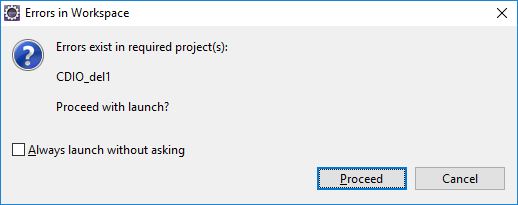
\includegraphics[width=0.5\paperwidth]{screenshots/error_box_eclipse.PNG}
    \caption{Error message in Eclipse}
    \label{fig:eclipse_error}
\end{figure}

\noindent That is no problem, just select \textit{Proceed}. The program should now execute. \\
Try to type "2" in the terminal, to check if the database works (it does not work). I get this error:\\
\texttt{[DBConnection::checkJDBCDriverExists]: Missing JDBC driver in the java project}\\
Luckily, this is an easy fix. In the folder, there is a \texttt{JDBC} driver that has not been added as a library properly.\\
Go to the project properties again (Right click on the project and select properties, or press ALT + Enter on the project) and follow the following steps:

\begin{enumerate}
    \item Go to \textit{Java Build Path}
    \item In the tabs in the top, select \textit{Libraries}
    \item Now that we are here, select \textit{APPLICATION\_HOME\_DIR/lib/junit-4.12.jar}. and click \textit{Remove}. It is used for Travis CI; eclipse has its own junit library.
    \item If \texttt{mysql\_connector-java-5.1-40-bin.jar} is there already, go to the \textbf{alternative step} below.
    \item Now, click \textit{Add JARs...}
    \item Go to CDIO\_del1
    \item Select \texttt{mysql\_connector-java-5.1.40-bin.jar} and click Ok.
    \item Click Ok again, and run the project.
\end{enumerate}
As before, we get an error, but it should not be a problem. Again, just proceed.\\
Now everything should work. 

\subsubsection{Alternative Step}

If you already have the \texttt{mysql\_connector-java-5.1-40-bin.jar} as a library in the project, follow this step. Select the .jar-file and click remove in the right side of the window. Then add it again, and proceed with the steps above.